%% JAIR submission version of "Precision Patches".
%% Body content is identical to the arXiv version (paper/precision_patches.tex);
%% only the class, title block, abstract structure, bibliography backend and the
%% Reproducibility Checklist appendix differ, per the JAIR Author Kit.
\documentclass[manuscript, screen, review]{jair}

\setcopyright{cc}
\acmDOI{10.1613/jair.1.xxxxx}

\JAIRAE{}
\JAIRTrack{}

%% The JAIR kit ships a BibLaTeX/biber setup; we use acmart's native
%% natbib + BibTeX path instead, which produces the same ACM author-year
%% reference format without requiring biber. Switch back to the kit's
%% biblatex block if your build environment has biber available.

%% Figures are drawn natively so they always render (no external image files).
\usepackage{pgfplots}
\pgfplotsset{compat=1.16}
\definecolor{okblue}{HTML}{0072B2}
\definecolor{okgreen}{HTML}{009E73}
\definecolor{okorange}{HTML}{E69F00}
\definecolor{okverm}{HTML}{D55E00}

\newcommand{\bpw}{bits/weight}
\newcommand{\code}[1]{\texttt{#1}}

\begin{document}

\title[Precision Patches]{Precision Patches: A Controlled Study of
Task-Conditional Quantization for Large Language Models}

\author{Mustafa Cem B\"uy\"ukalpelli}
\authornote{Corresponding Author.}
\email{mustafacembuyukalpelli@gmail.com}
\affiliation{%
  \institution{Independent Researcher}
  \country{Turkey}
}
\renewcommand{\shortauthors}{B\"uy\"ukalpelli}

\begin{abstract}
{\bf Background:}
Post-training quantization compresses a large language model once, into a
single static artifact whose quality is fixed across all downstream uses. If
\emph{which} weights matter most depends on the task being served, a shared
base plus small swappable ``precision patches'' should beat a single static
model.

{\bf Objectives:}
We test that premise end to end: whether weight sensitivity is genuinely
task-dependent, whether task-conditional patches beat strong null hypotheses at
matched memory, and whether any patch configuration improves on ordinary
uniform quantization.

{\bf Methods:}
A controlled study on Qwen2.5 (0.5B, with structural diagnostics at 1.5B and
7B) with full-surface quantization of all seven linear projection types, a
split-half noise-ceiling methodology for sensitivity claims, a closed-form
activation-space correction that reuses the quantizer's own Hessian, and
matched-memory comparisons throughout, evaluated in both perplexity and GSM8K
accuracy.

{\bf Results:}
Sensitivity is task-dependent, and MLP layers carry substantially more
task-specific structure than attention. The patch mechanism is real: patches
beat per-layer-type mixed precision by roughly $2\times$ at matched memory
($p{=}1.000$ on all four tasks), and storing corrections at 3 bits rather than
\code{fp16} is worth $2.13\times$. However, the task \emph{conditioning} does
not pay---mismatched patches transfer as well as matched ones and a single
universal patch suffices---and uniform quantization remains the better use of a
bit on absolute quality. Most consequentially, an end-to-end \emph{learned}
patch reaches perplexity parity with uniform 4-bit at 19\% lower memory yet
collapses to 8.5\% GSM8K accuracy, below the unpatched base's 12.5\%.

{\bf Conclusions:}
The deployable win is a cheap mixed-precision base, not task swapping. The
broader lesson is methodological: perplexity understates quantization damage by
roughly an order of magnitude ($+2.8\%$ perplexity costs $-31.9\%$ accuracy)
and, for a perplexity-optimised patch, inverts the ranking outright. Quality
claims for sub-4-bit quantization should be validated on downstream accuracy.
All code, results, and four explicitly retracted claims are released.
\end{abstract}

\maketitle

\section{Introduction}

Quantization is the dominant lever for deploying large language models (LLMs)
under memory constraints. Standard post-training quantization (PTQ) methods
such as GPTQ~\cite{frantar2022gptq} and AWQ~\cite{lin2023awq} compress a model
once into a single static artifact whose quality is fixed across all
downstream uses. This is efficient but leaves value on the table if
\emph{which} weights matter most depends on the task the model is serving.

We investigate a simple alternative that borrows the deployment story of
parameter-efficient adapters~\cite{hu2021lora}. Ship one aggressively
quantized base model and, alongside it, small \emph{precision patches}: for a
given task, a subset of weight groups is restored to higher precision, chosen
from task-specific calibration data. Serving a coding workload loads the code
patch; a math workload swaps in the math patch. Unlike LoRA, no new parameters
are introduced---a patch only recovers information the full-precision model
already had. The scientific question underneath the engineering is whether
quantization sensitivity is task-dependent enough to make this worthwhile.

We study this question exhaustively and report an honest, nuanced answer. The
mechanism works and is statistically decisive against strong null hypotheses,
but two things it is widely assumed to deliver, it does not. It does not beat
the simplest baseline---spending the same bits uniformly---on absolute quality.
And the \emph{task} conditioning, the premise of swappability, does not pay: a
single universal patch works as well as per-task ones, and mismatched patches
transfer nearly as well as matched ones. What genuine value remains is narrow
and geometric: integer-only uniform quantization cannot occupy the memory band
between consecutive bit-widths, and patches (together with mixed precision)
fill it.

Along the way we surface two measurement findings that we believe matter
beyond this paper: perplexity dramatically understates the downstream damage
of quantization, and calibration-seed variance is large enough (up to 3.35\%
relative) that many small single-seed ``wins'' in this line of work are
unproven.

\paragraph{Contributions.}
\begin{itemize}
  \item A \emph{task-sensitivity atlas} with a split-half noise-ceiling
    methodology that makes ``high overlap'' interpretable, establishing that
    quantization sensitivity is task-dependent but that MLP layers carry the
    task-specific signal while attention is largely task-universal
    (Sec.~\ref{sec:atlas}).
  \item A \emph{closed-form activation-space correction} for patch values that
    reuses the quantizer's own Hessian and provably dominates naive
    weight restoration, resolving a coupling problem specific to
    compensated quantizers like GPTQ (Sec.~\ref{sec:method}).
  \item A rigorous, \emph{matched-memory} characterization of the
    quality/memory Pareto frontier from 2.25 to 5.25 \bpw{}, in both
    perplexity and GSM8K accuracy, including a battery of ablations and four
    explicitly retracted claims (Secs.~\ref{sec:results}--\ref{sec:negative}).
  \item The finding that \emph{perplexity understates quantization damage
    $\sim$10$\times$ relative to accuracy}, and a first quantification of
    calibration-seed variance (Sec.~\ref{sec:caveats}).
  \item A cautionary demonstration that an end-to-end \emph{learned}
    (distillation-trained) patch reaches perplexity parity with uniform-4 at
    lower memory yet \emph{collapses} on task accuracy, below even the
    unpatched base---perplexity here does not merely understate damage, it
    inverts the ranking (Sec.~\ref{sec:learned}).
\end{itemize}

\section{Related Work}

\paragraph{Post-training quantization.} GPTQ~\cite{frantar2022gptq} quantizes
weights column-by-column while compensating unquantized columns for the
induced error, using a Hessian estimated from calibration activations.
AWQ~\cite{lin2023awq} scales salient channels by activation magnitude before
round-to-nearest. Both target a single static model. We build directly on the
GPTQ formulation and reuse its Hessian for patch construction.

\paragraph{Mixed-precision and outlier-aware quantization.} A body of work
observes that a small fraction of weights or channels dominate quantization
error and protects them at higher precision: LLM.int8()~\cite{dettmers2022int8}
keeps outlier channels in \code{fp16}, SpQR~\cite{dettmers2023spqr} and
SqueezeLLM~\cite{kim2023squeezellm} isolate outlier weights. These allocate
precision non-uniformly but produce one static model with no task
conditioning. Our patches are group-level, task-conditional, and swappable; we
find, however, that much of their benefit coincides with per-layer-type mixed
precision (Sec.~\ref{sec:vsmixed}), which situates the contribution precisely.

\paragraph{Task-aware quantization.} Closest to our motivation is
TAQ~\cite{levi2025taq}, a training-free mixed-precision PTQ framework that
scores \emph{layer} importance from task-specific calibration prompts and
allocates higher precision to task-relevant layers, producing one quantized
model per task. Our design differs in artifact and granularity: a single shared
base plus $N$ cheap swappable patches, at weight-group rather than layer
granularity. It also differs in what we conclude---we find that the task
conditioning itself does not pay (Sec.~\ref{sec:crosstask}), which a
per-task-model formulation cannot easily reveal, because it never asks whether
one \emph{universal} artifact would have sufficed. Our controlled comparisons
against a task-\emph{calibrated} base (Sec.~\ref{sec:vsmixed}) and a pooled
patch are, to our knowledge, not standard and are essential for isolating what
task conditioning actually buys.

\paragraph{Adapters.} Precision patches are structurally analogous to
LoRA~\cite{hu2021lora}: a frozen base plus small swappable task modules. The
distinction is that a restored patch adds no parameters and stores a quantized
residual rather than a learned low-rank update. Our main comparison to uniform
quantization uses such training-free patches to keep the setting clean; we then
test a \emph{learned} (distillation-trained) variant in isolation
(Sec.~\ref{sec:learned}), where it exposes a metric trap rather than a gain.

\section{Method}
\label{sec:method}

\subsection{Setup and notation}
Weights of a linear layer are $W \in \mathbb{R}^{d_\text{out}\times d_\text{in}}$.
We use group-wise quantization with group size $g{=}128$: contiguous runs of
$g$ input-dimension weights per output row share one asymmetric scale and
zero-point. A \emph{group} is the atomic patch unit, aligned to the
quantization grid so that patching a group never disturbs a neighbor's
scales. Let $Q(W)$ denote the quantized base and $R = W - Q(W)$ the residual.
Calibration activations $X$ define the layer Hessian $H = X^\top X$.

A patch selects a set $S$ of groups and stores a correction $\Delta$ supported
on $S$; the served weight is $Q(W) + \Delta$. Two design choices define a
patch: \emph{which} groups (the mask) and \emph{what} correction values.

\subsection{Task-sensitivity scoring}
We score each group by its contribution to activation-space error. For group
$G$ we use an OBS/OBC-style~\cite{lecun1989obd,frantar2022gptq} saliency: the
error reduction achievable by optimally correcting that group in isolation,
\begin{equation}
  s(G) \;=\; (Hr)_G^\top \, (H_{GG})^{-1} \, (Hr)_G,
  \label{eq:obs}
\end{equation}
which is exactly the drop in $\lVert X(W - Q(W) - \Delta)\rVert_F^2$ obtainable
by correcting only $G$. Scores are computed from task-specific $H$, so
selection is task-conditional. Equation~\eqref{eq:obs} is stated in the same
units as the objective the patch optimizes, unlike magnitude- or
activation-only heuristics.

\subsection{Closed-form activation-space correction}
The naive patch restores selected groups to their original values,
$\Delta_S = R_S$. This is optimal only if the base is an unbiased per-weight
approximation---which a GPTQ base is \emph{not}, because its error compensation
has already redistributed each group's quantization error into surrounding
weights. Restoring a group then removes an error the rest of the matrix is
still compensating for. Empirically, patching a GPTQ base with restored values
\emph{hurt} in 13 of 16 configurations.

We instead solve for the correction that minimizes activation-space
reconstruction error against the base that actually exists. For a fixed mask
$S$, minimizing $\lVert X(R - \Delta)\rVert_F^2$ subject to
$\mathrm{supp}(\Delta)\subseteq S$ has, per output row, the closed form
\begin{equation}
  \Delta_S \;=\; (H_{SS})^{-1}\,(Hr)_S ,
  \label{eq:solve}
\end{equation}
where $H$ is exactly the Hessian GPTQ already accumulates. No gradient descent
is required. Restoration is the special case $\Delta_S = R_S$, so
Eq.~\eqref{eq:solve} strictly dominates it: it optimizes over a space
containing the naive solution as one point. Because the objective references
the actual base, compensation ceases to be a problem to avoid and becomes a
term the solve absorbs. This alone raised the fraction of configurations in
which patching helps a GPTQ base from 3/16 to 20/48.

\subsection{Variable-bit patch storage}
\label{sec:varbit}
Earlier iterations of this idea, and much outlier-protection work, restore
selected weights to \code{fp16}. On a 3-bit base that spends $+12.75$
\bpw{} on each patched weight. But the quantization bit-scaling law---each
added bit removes $\approx 79\%$ of remaining error, matching the
$\Delta^2/12$ theory that predicts $75\%$---implies most of the benefit lies in
the first few added bits. We therefore quantize the \emph{solved} correction
$\Delta$ to $b_p$ bits with the same group-wise machinery as the base. The
\code{fp16} patch is the special case $b_p{=}16$, making prior designs a
single point on a sweep. At matched \emph{bytes}, the fair question is whether
to patch few groups precisely or many groups coarsely.

\subsection{Mask encoding}
A patch must record which groups it stores. An explicit $(\text{row},
\text{group})$ index costs 8~bytes against $\approx$52~bytes of 3-bit payload
per group---13\% overhead, paid per group. A dense bitmap over all groups costs
a flat $\lceil |G|/8\rceil$ bytes and wins above $\approx$1.5\% coverage; at the
$\sim$22\% coverage these patches run at, it frees $\sim$12\% of the budget,
buying $\sim$14\% more coverage.

\section{Experimental Setup}
\label{sec:setup}

\paragraph{Models and surface.} All models come from the Qwen2.5-Instruct
family. Every headline result---the sensitivity atlas
(Sec.~\ref{sec:atlas}), cross-task transfer
(Sec.~\ref{sec:crosstask}), the Pareto frontier and precision/allocation
ablations (Sec.~\ref{sec:results}), the learned-patch experiment
(Sec.~\ref{sec:learned}), the measurement caveats (Sec.~\ref{sec:caveats}), and
all GSM8K accuracy---is on \textbf{Qwen2.5-0.5B-Instruct}. The scale diagnostic
(Sec.~\ref{sec:scale}) alone additionally uses \textbf{Qwen2.5-1.5B-Instruct}
and \textbf{Qwen2.5-7B-Instruct}; the 7B model, which exceeds the 6\,GB test
GPU, is quantized and scored one transformer block at a time (peak 0.59\,GB).
Table~\ref{tab:models} lists the model per experiment. Unless stated,
experiments quantize the \emph{full surface}: all seven linear projection types
(\code{q,k,v,o,gate,up,down}), 358M weights for the 0.5B model. Prior iterations
that quantized only \code{o\_proj} and \code{down\_proj} (35\% of weights) left
the rest in \code{fp16} and thereby inflated quality; all headline numbers here
use the full surface.

\begin{table}[t]
\centering
\caption{Model used per experiment. All quality/accuracy claims are on
Qwen2.5-0.5B-Instruct; only the structural scale diagnostic uses larger models.}
\label{tab:models}
\begin{tabular}{ll}
\toprule
Experiment / section & Model(s) \\
\midrule
Task-sensitivity atlas (\S\ref{sec:atlas}) & Qwen2.5-0.5B-Instruct \\
Cross-task transfer (\S\ref{sec:crosstask}) & Qwen2.5-0.5B-Instruct \\
Pareto frontier, PPL + GSM8K (\S\ref{sec:frontier}) & Qwen2.5-0.5B-Instruct \\
Patch precision / allocation (\S\ref{sec:precision}--\ref{sec:vsmixed}) & Qwen2.5-0.5B-Instruct \\
Learned patch + GSM8K (\S\ref{sec:learned}) & Qwen2.5-0.5B-Instruct \\
Measurement caveats (\S\ref{sec:caveats}) & Qwen2.5-0.5B-Instruct \\
Scale diagnostic (\S\ref{sec:scale}) & Qwen2.5-0.5B / 1.5B / 7B-Instruct \\
\bottomrule
\end{tabular}
\end{table}

\paragraph{Data.} Four tasks: code (MBPP; calibration from CodeParrot), math
(GSM8K), knowledge (ARC-Easy), and general text (WikiText-2). Calibration uses
2048-token sequences reaching 26--54 activation samples per Hessian dimension;
we verified calibration/evaluation disjointness by 8-gram overlap
($\le$3\%). \emph{Hessian conditioning is reported for every $H$-dependent step
and is a prerequisite}: an early positive result (a ``code exception'') was
retracted after we traced it to a rank-deficient Hessian at $<$1 sample per
dimension.

\paragraph{Metrics.} Perplexity on held-out task text, and GSM8K exact-match
accuracy (200 problems, 4-shot, greedy). Significance by paired bootstrap
($N{=}4000$) over evaluation items. \emph{Every configuration is reported with
its effective \bpw{}}; no comparison is made at unequal cost. This discipline
was necessary: three distinct confounds in preliminary work arose from
comparing configurations at unequal memory. One further caution applies to the
reader: absolute perplexities are \emph{not} comparable across our tables,
because evaluation sequence length differs between experiments (2048 tokens in
the frontier and ablation runs, 256 in the training-based runs, which must fit
a 6\,GB GPU alongside a teacher). Perplexity rises with shorter contexts, so a
configuration can read $3.83$ in one table and $5.51$ in another. Every
comparison we draw---and every significance test---is \emph{within} a single
run, where all configurations share an identical evaluation.

\paragraph{Reproducibility.} Fake quantization (dequantized values held in
\code{fp16}); we measure memory and quality, and claim no wall-clock speedup.
Models larger than VRAM are handled by block-streaming quantization (peak
0.59~GB for the 7B model on a 6~GB GPU). Code and all result files are
released.

\section{Results}
\label{sec:results}

\subsection{Task sensitivity is real, and lives in the MLP}
\label{sec:atlas}
We first ask whether sensitivity is task-dependent at all. The raw overlap of
the top-1\% most sensitive groups across tasks is 65--80\% (Jaccard), which
sounds high in isolation. It becomes interpretable only against a
\emph{noise ceiling}: splitting one task's calibration set in half and
re-scoring yields within-task overlap of $0.970$. Two samples of the same task
agree at 97\%; different tasks agree at 65--80\%; random selection agrees at
$0.5\%$. The go/no-go signal (ceiling minus cross-task overlap) is $0.246$,
comfortably above a pre-registered threshold of $0.15$.

A secondary finding: attention layers are far more task-universal than MLP
layers (mean cross-task overlap $0.750$ vs.\ $0.492$). Task-specific structure
concentrates in the MLP. This foreshadows Sec.~\ref{sec:vsmixed}, where
much of the patch benefit turns out to coincide with a coarse
attention-vs-MLP precision split.

\subsection{Task conditioning barely pays: a universal patch suffices}
\label{sec:crosstask}
Sensitivity being task-dependent (above) does not imply that a task-\emph{matched}
patch outperforms a task-agnostic one. We test this directly---the natural
expectation being that, say, a math patch should transfer poorly to code. It
does not. Table~\ref{tab:crosstask} evaluates each fully self-contained patch
(mask \emph{and} values from one task's calibration) on every task. Off-diagonal
(mismatched) entries are not systematically worse than the diagonal; on the code
column, the math and chat patches (6.352, 6.320) in fact edge out code's own
patch (6.467). Averaged over the grid, a single \emph{pooled} patch built from
generic mixed-task data wins as often as any task-specific patch, and a
task-matched patch beats the pooled patch significantly only in a narrow regime
(3-bit base, small budgets $k\!\in\!\{1,2\}\%$, on math/knowledge/chat; never
convincingly on code).

\begin{table}[t]
\centering
\caption{Cross-task patch transfer (perplexity, OBS mask, $k{=}5\%$; rows =
task the patch was built from, columns = evaluation task; lower is better).
Mismatched patches perform on par with matched ones---a math patch on code
(6.352) beats code's own patch (6.467). Task conditioning's \emph{payoff} is
weak even though sensitivity is task-dependent, so a single universal patch
suffices and the ``swappable per-task'' motivation is not supported.}
\label{tab:crosstask}
\begin{tabular}{lrrrr}
\toprule
patch $\backslash$ eval & code & math & knowledge & chat \\
\midrule
code            & 6.467 & 6.606 & 8.176 & 31.813 \\
math            & 6.352 & 6.505 & 7.964 & 31.316 \\
knowledge       & 6.377 & 6.524 & 7.931 & 31.514 \\
chat            & 6.320 & 6.597 & 8.173 & 31.012 \\
pooled (univ.)  & 6.513 & 6.489 & 7.900 & 31.155 \\
\midrule
base (no patch) & 6.102 & 6.770 & 8.587 & 32.444 \\
\bottomrule
\end{tabular}
\end{table}

This is the study's most direct negative result about the original motivation:
a shared base plus \emph{one} universal patch captures essentially all the
benefit, so there is little reason to ship or swap per-task patches. The
mechanism is task-conditional in its \emph{scoring} (Sec.~\ref{sec:atlas}) but
not, in practice, in its \emph{payoff}.

\subsection{The Pareto frontier, measured in accuracy}
\label{sec:frontier}
Table~\ref{tab:frontier} and Fig.~\ref{fig:frontier} report GSM8K accuracy
across configurations spanning 2.25--5.25 \bpw{}. Three regimes emerge.

\begin{table}[t]
\centering
\caption{GSM8K accuracy across the memory frontier (Qwen2.5-0.5B, full
surface, 200 problems, 4-shot). ``mix$XY$'' = attention at $X$ bits, MLP at $Y$
bits; ``+pb3'' = a 3-bit precision patch. \textbf{Bold} marks the Pareto
frontier. Uniform quantization exists only at integer bit-widths, leaving the
shaded interior bands to mixed precision and patches.}
\label{tab:frontier}
\begin{tabular}{lrr}
\toprule
Configuration & \bpw{} & GSM8K acc. \\
\midrule
uniform 2-bit & 2.250 & 1.0\% \\
mix32 & 2.373 & 1.5\% \\
mix32 + pb3 & 3.198 & 0.5\% \\
\textbf{uniform 3-bit} & \textbf{3.250} & \textbf{8.5\%} \\
\textbf{mix43} & \textbf{3.373} & \textbf{12.5\%} \\
mix43 + pb3 & 4.198 & 23.0\% \\
\textbf{uniform 4-bit} & \textbf{4.250} & \textbf{23.5\%} \\
\textbf{mix54} & \textbf{4.373} & \textbf{31.0\%} \\
mix54 + pb3 & 5.198 & 30.5\% \\
\textbf{uniform 5-bit} & \textbf{5.250} & \textbf{34.5\%} \\
\midrule
fp16 (reference) & 16.000 & 34.5\% \\
\bottomrule
\end{tabular}
\end{table}

\begin{figure}[t]
\centering
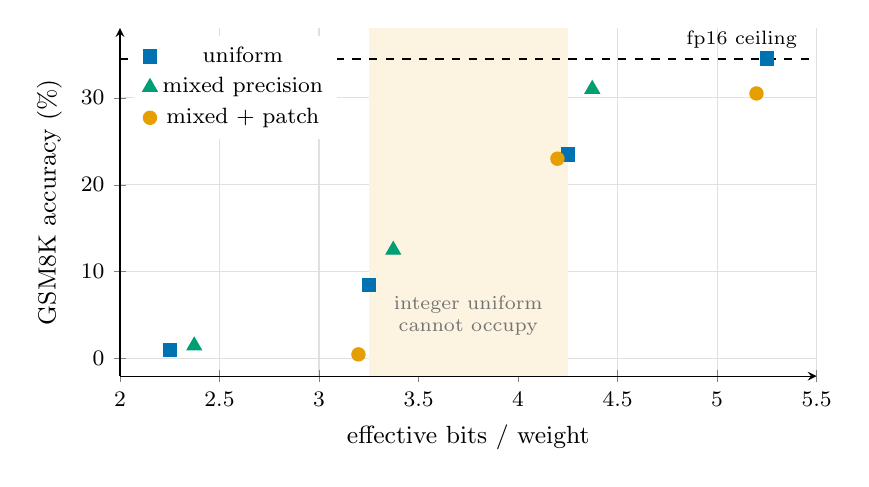
\begin{tikzpicture}
\begin{axis}[
  width=0.86\linewidth, height=6.0cm,
  xlabel={effective bits / weight}, ylabel={GSM8K accuracy (\%)},
  xmin=2.0, xmax=5.5, ymin=-2, ymax=38,
  grid=major, grid style={black!12},
  axis lines=left, tick label style={font=\footnotesize},
  label style={font=\small},
  legend style={draw=none, font=\footnotesize, at={(0.02,0.98)}, anchor=north west},
]
\fill[okorange!12] (axis cs:3.25,-2) rectangle (axis cs:4.25,38);
\addplot[black, dashed, thick, forget plot] coordinates {(2,34.5) (5.5,34.5)};
\node[font=\scriptsize, anchor=south east] at (axis cs:5.45,34.6) {fp16 ceiling};
\addplot[only marks, mark=square*, mark size=2.4pt, okblue]
  coordinates {(2.25,1.0) (3.25,8.5) (4.25,23.5) (5.25,34.5)};
\addlegendentry{uniform}
\addplot[only marks, mark=triangle*, mark size=3pt, okgreen]
  coordinates {(2.373,1.5) (3.373,12.5) (4.373,31.0)};
\addlegendentry{mixed precision}
\addplot[only marks, mark=*, mark size=2.4pt, okorange]
  coordinates {(3.198,0.5) (4.198,23.0) (5.198,30.5)};
\addlegendentry{mixed + patch}
\node[font=\scriptsize, text=black!55, align=center] at (axis cs:3.75,5)
  {integer uniform\\cannot occupy};
\end{axis}
\end{tikzpicture}
\caption{The quality/memory frontier in \emph{GSM8K accuracy} (not perplexity),
on Qwen2.5-0.5B-Instruct. Uniform quantization exists only at integer
bit-widths (squares); the shaded $3.25$--$4.25$ \bpw{} band is reachable only by
mixed precision (triangles) and patches (circles). At the integer rungs uniform
is competitive---\code{mix43+patch} $23.0\%$ vs.\ uniform-4 $23.5\%$, a tie at
lower memory; below $3.25$ \bpw{} every configuration collapses to chance.}
\label{fig:frontier}
\end{figure}

\textbf{Below 3.25 \bpw{}: nothing works.} Every configuration on a 2-bit base
scores at chance (0.5--1.5\%). The 2-bit base is too destroyed for any
affordable correction to rescue; \code{mix32+pb3} at 3.198 \bpw{} is actually
\emph{worse} than plain uniform 3-bit, i.e.\ spending bits to patch a dead base
is counterproductive. We caution that perplexity badly obscures this: relative
to \code{fp16}, uniform 2-bit is $\sim$22{,}000$\times$ perplexity, and a
configuration ``closing 98.6\% of the perplexity gap'' still sits at
$\sim$300$\times$---a dead model that the ratio flatters.

\textbf{The usable frontier (3.25--5.25 \bpw{}) is owned by mixed precision and
patches at every interior point.} Because uniform quantization is integer-only,
it simply does not exist between 3.25 and 4.25 \bpw{}; the band belongs to
\code{mix43} and \code{mix43+pb3}.

\textbf{At the integer rungs, uniform is competitive, and a patch just reaches
it at slightly lower memory.} \code{mix43+pb3} (4.198 \bpw{}) reaches 23.0\%
versus uniform 4-bit's 23.5\% (4.250 \bpw{})---a statistical tie ($p{=}0.406$
by paired bootstrap) at lower memory, and the tie holds in perplexity too. This
is the one deployable positive configuration the study produces, and it holds
with a \emph{universal} patch, not only a task-specific one: replacing the
per-task patch with a pooled-calibration patch on the same base gives $17.0\%$
vs.\ uniform-4's $17.5\%$ ($p{=}0.47$, indistinguishable) at $4.198$ vs.\ $4.250$
\bpw{} in a separate run---consistent with Sec.~\ref{sec:crosstask} that task
conditioning is unnecessary. The saving is real but modest ($\sim$1\% of
memory), and the efficient ingredient is the mixed-precision \emph{base}: it
alone reaches $16.0\%$ at $3.37$ \bpw{}, and the patch spends $0.8$ further
bits to add a single accuracy point.

\subsection{Patch precision: 3-bit, not \code{fp16}}
\label{sec:precision}
Storing the solved correction at 3 bits rather than \code{fp16}, at matched
bytes, closes $46.9\%$ of the quantization gap versus $22.0\%$ for
\code{fp16}---a $2.13\times$ improvement, significant on all four tasks
($p{=}1.000$). This matches the activation-space prediction and validates the
bit-scaling argument of Sec.~\ref{sec:varbit}. The optimum is interior:
2-bit patches are \emph{worse} than 3-bit (catastrophically so on attention),
so ``lower is always better'' does not hold.

\subsection{Patches are not merely mixed precision}
\label{sec:vsmixed}
Sec.~\ref{sec:atlas} showed task structure concentrates in the MLP, and
attention tolerates less error. This raises the strongest null hypothesis: are
patches an expensive way to rediscover ``attention needs more bits than MLP,''
which plain per-layer-type mixed precision achieves with no Hessian solve, no
mask, and no indices? We test this at matched memory. At $\approx$4.03 versus
4.075 \bpw{}, patches close $46.9\%$ of the gap against mixed precision's
$24.4\%$---nearly $2\times$, at $p{=}1.000$ on all four tasks. Whatever the
saliency scores select is substantially finer-grained than a layer-type split.

We also tested the converse charitable hypothesis---that allocation was the
bug and forcing budget onto attention would help---and it failed: proportional
top-$k$ and attention-weighted allocation are indistinguishable, and pushing
100\% of budget onto attention collapses performance (attention is only
$\sim$12\% of the full surface).

\subsection{The verdict against uniform, and per-bit efficiency}
Despite the above, uniform 4-bit wins on \emph{absolute} quality: 89.3\% of the
perplexity gap closed versus the best patch config's 67.3\% at comparable cost,
$p{=}0.000$ on three of four tasks (math is the tie). What patches and mixed
precision win instead is \emph{per-bit efficiency} and \emph{frontier
coverage}. On the full surface, upgrading attention by one bit costs only
0.123 \bpw{} and recovers 41.2\% of the gap---the single most byte-efficient
intervention we measured, roughly $4\times$ uniform-4-bit's efficiency per
bit. The practical recommendation is therefore explicit: for maximum quality
at $\approx$4.25 \bpw{}, use uniform 4-bit; for any memory budget between
integer bit-widths, a mixed-precision base with an optional 3-bit patch
dominates.

\subsection{Scale: no free lunch}
\label{sec:scale}
We measured the uniform-vs-patch per-bit efficiency ratio at matched depth on
attention layers across 0.5B, 1.5B, and 7B, \emph{using the best variable-bit
patch at each scale} so the comparison is design-matched. It is flat:
$1.05\times$, $0.97\times$, $1.12\times$ respectively (values $<1$ favor
patches). Layer-to-layer variance within a single model exceeds the variation
across a $14\times$ range of model sizes. An earlier report of a
``scale-gated'' effect was retracted: it compared \code{fp16} patches at 0.5B
against a hybrid at 1.5B, i.e.\ different designs, not different scales---the
same trap that makes the design-matching above essential.

\section{What Did Not Work}
\label{sec:negative}
We ran and rejected several ideas with pre-registered promotion rules
(a $\geq$5\% relative improvement at matched bytes on a majority of probe
layers). We report them because negative results at matched memory are the
main safeguard against the metric confounds that dogged this project.

\begin{itemize}
  \item \textbf{Solve/quantize iteration} (alternate solving and re-quantizing
    the residual): rejected, 0/12 probes. Two 3-bit rounds is $\approx$6-bit
    fidelity on half the coverage, and 6-bit patches already lose to 3-bit.
  \item \textbf{Residual-aware re-selection} (spend half the budget, re-score
    against the partial correction, spend the rest): rejected, 1/12 probes.
  \item \textbf{Attention-weighted budget allocation}: no effect versus
    proportional top-$k$ (Sec.~\ref{sec:vsmixed}).
  \item \textbf{Scaling past 0.5B} as a route to beating uniform: the frontier
    curve is flat (Sec.~\ref{sec:scale}).
\end{itemize}

A single positive method change survived: \textbf{bitmap mask encoding}
(Sec.~\ref{sec:method}), promoted at 12/12 probes in activation space. We note
in Sec.~\ref{sec:caveats} that its perplexity gain is partly within seed noise.

The unifying explanation for the pattern is that, at a fixed byte budget,
\emph{coverage dominates fidelity}. Every idea that traded coverage for
precision (fp16 patches, iteration, 2-bit patches) lost; every idea that bought
coverage (3-bit patches, bitmap) won.

\section{Learned patches: a perplexity mirage}
\label{sec:learned}

Every patch above only \emph{restores} information already present in the fp16
model: the closed-form solve reconstructs each layer's output locally, so a
patch can at best claw the quantized model back toward fp16. A patch
\emph{trained} end-to-end against the fp16 teacher can, in principle, do more:
compensate for error propagating \emph{across} layers, since the loss is on the
final logits. We test this---and it produces the sharpest cautionary result in
the paper.

\paragraph{Setup.} On the mixed attention@4/MLP@3 base (frozen), we place a
sparse trainable residual on the top-$5\%$ \code{down\_proj} groups (OBS
selection; Fisher/task-loss-gradient selection was tried and found
\emph{worse}). The residual is trained with a distillation loss
$\mathrm{KL}(p_\text{fp16}\,\|\,p_\text{student})$ on task calibration text
(up to 128 sequences, 12 epochs), then quantized to 3 bits and stored exactly
like a solved patch, at identical bytes.

\paragraph{Perplexity says: breakthrough.} Trained to convergence on math, the
learned patch reaches \emph{perplexity parity} with uniform-4 at 19\% lower
memory (Table~\ref{tab:learned}, 4.77 vs.\ 4.73 at 3.43 vs.\ 4.25 \bpw{}). It
beats the restored patch decisively---in a matched run where the restored patch
scored $5.97$ against a base of $5.85$, i.e.\ restoration \emph{hurt} while the
learned patch helped---quantizing the trained delta to 3 bits is free
($<0.02$ ppl), and the improvement grows monotonically with training data
($5.11 \to 4.97 \to 4.77$). By every perplexity measure this is the win the
whole method was after.

\paragraph{Accuracy says: worse than doing nothing.} It is not. On GSM8K
exact-match (200 problems, 4-shot), the same learned patch scores
\textbf{8.5\%}---below the unpatched base (12.5\%) and far below uniform-4
(23.5\%), $p{=}0.000$. The KL distillation lowered perplexity by matching the
teacher's output \emph{distribution} on calibration text while \emph{destroying}
the reasoning GSM8K requires; training \emph{harder} for lower perplexity made
task accuracy \emph{worse}.

\begin{table}[t]
\centering
\caption{The learned patch reaches perplexity parity with uniform-4 at lower
memory, yet collapses on GSM8K accuracy---below even the unpatched base. This
is the perplexity/accuracy divergence of Sec.~\ref{sec:caveats} in its most
extreme form: on perplexity the learned patch looks like a clear win; on
accuracy it is worse than doing nothing. All rows come from a single run, so
they are directly comparable; base and uniform-4 accuracies match the
independent measurements of Sec.~\ref{sec:frontier} exactly. Absolute
perplexities are not comparable across tables in this paper because evaluation
sequence length differs between runs (see Sec.~\ref{sec:setup}); every
comparison we draw is within a run.}
\label{tab:learned}
\begin{tabular}{lrrr}
\toprule
config (math) & \bpw{} & perplexity & GSM8K acc. \\
\midrule
base (mixed attn@4/MLP@3) & 3.37 & 5.51 & 12.5\% \\
\textbf{learned patch} & \textbf{3.43} & \textbf{4.77} & \textbf{8.5\%} \\
uniform-4 & 4.25 & 4.73 & 23.5\% \\
fp16 & --- & 4.49 & 34.5\% \\
\bottomrule
\end{tabular}
\end{table}

\begin{figure}[t]
\centering
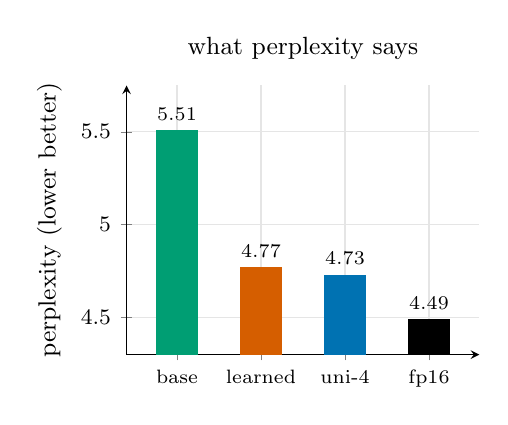
\begin{tikzpicture}
\begin{axis}[
  width=0.5\linewidth, height=5.0cm,
  ymin=4.3, ymax=5.75, ylabel={perplexity (lower better)},
  xmin=0.4, xmax=4.6, xtick={1,2,3,4},
  xticklabels={base, learned, uni-4, fp16},
  x tick label style={font=\scriptsize}, tick label style={font=\footnotesize},
  label style={font=\small}, title={\small what perplexity says},
  grid=major, grid style={black!10}, axis lines=left,
  nodes near coords, nodes near coords style={font=\scriptsize},
  every node near coord/.append style={/pgf/number format/fixed,/pgf/number format/precision=2},
]
\addplot[ybar, bar width=15pt, bar shift=0pt, fill=okgreen, draw=none] coordinates {(1,5.51)};
\addplot[ybar, bar width=15pt, bar shift=0pt, fill=okverm,  draw=none] coordinates {(2,4.77)};
\addplot[ybar, bar width=15pt, bar shift=0pt, fill=okblue,  draw=none] coordinates {(3,4.73)};
\addplot[ybar, bar width=15pt, bar shift=0pt, fill=black,   draw=none] coordinates {(4,4.49)};
\end{axis}
\end{tikzpicture}\hfill
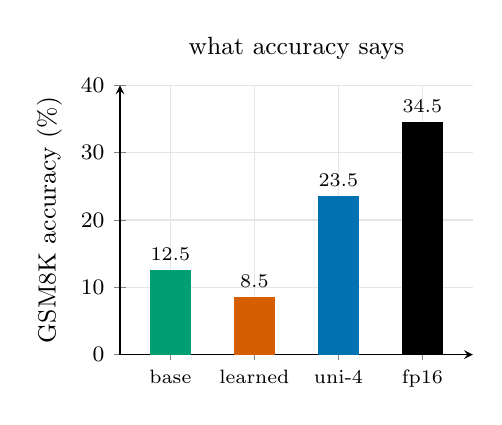
\begin{tikzpicture}
\begin{axis}[
  width=0.5\linewidth, height=5.0cm,
  ymin=0, ymax=40, ylabel={GSM8K accuracy (\%)},
  xmin=0.4, xmax=4.6, xtick={1,2,3,4},
  xticklabels={base, learned, uni-4, fp16},
  x tick label style={font=\scriptsize}, tick label style={font=\footnotesize},
  label style={font=\small}, title={\small what accuracy says},
  grid=major, grid style={black!10}, axis lines=left,
  nodes near coords, nodes near coords style={font=\scriptsize},
  every node near coord/.append style={/pgf/number format/fixed,/pgf/number format/precision=1},
]
\addplot[ybar, bar width=15pt, bar shift=0pt, fill=okgreen, draw=none] coordinates {(1,12.5)};
\addplot[ybar, bar width=15pt, bar shift=0pt, fill=okverm,  draw=none] coordinates {(2,8.5)};
\addplot[ybar, bar width=15pt, bar shift=0pt, fill=okblue,  draw=none] coordinates {(3,23.5)};
\addplot[ybar, bar width=15pt, bar shift=0pt, fill=black,   draw=none] coordinates {(4,34.5)};
\end{axis}
\end{tikzpicture}
\caption{The learned-patch mirage (Qwen2.5-0.5B-Instruct, math). \emph{Left:} by
perplexity, the learned patch (4.77) is second only to fp16 and essentially ties
uniform-4 (4.73) at lower memory. \emph{Right:} by GSM8K accuracy it is the
worst usable configuration---below the unpatched base (8.5\% vs.\ 12.5\%). KL
distillation optimised the output distribution on calibration text while
destroying the reasoning the task needs; here perplexity does not understate
damage, it \emph{inverts} the ranking.}
\label{fig:mirage}
\end{figure}

The lesson is not that learned patches are inherently useless---a
distillation objective aligned with the downstream task, rather than raw KL on
generic text, might behave differently. It is that \emph{a perplexity-optimised
patch can be actively harmful to task capability}, and that any patch method
optimised or evaluated on perplexity alone---including, potentially, some in
the broader quantization literature---may report gains that reverse under
accuracy. It is the strongest possible vindication of Sec.~\ref{sec:caveats}:
here perplexity did not merely understate damage, it pointed the opposite way.

\paragraph{Scope.} This trains a residual (QLoRA-adjacent), so ``no additional
training'' is no longer a property of the method; the comparison to uniform
quantization remains fair (matched bits). The result is single seed, 0.5B,
\code{down\_proj} only, under a 6\,GB training budget. We tested the simplest
KL-only variant; a task-loss-aligned distillation objective, joint base/patch
optimization, activation quantization, and input-conditional precision are all
untested, and one of them may yet yield a learned patch whose perplexity gain
survives on accuracy. What this experiment establishes is narrower and, we
think, more useful as a warning than as a method: end-to-end perplexity
distillation can buy a perplexity win that is an accuracy loss.

\section{Measurement Caveats}
\label{sec:caveats}

\subsection{Perplexity understates quantization damage}
The most broadly relevant finding is a discrepancy between metrics.
Table~\ref{tab:pplacc} contrasts perplexity increase with GSM8K accuracy loss
for the same models. A $+2.8\%$ perplexity increase (uniform 4-bit) costs
$-31.9\%$ accuracy; a $+31.3\%$ increase (uniform 3-bit) costs $-75.4\%$.
Perplexity moves a few percent where accuracy moves tens of percent.

\begin{table}[t]
\centering
\caption{Perplexity vs.\ GSM8K accuracy degradation on the math task, same
models. Config \emph{ordering} is preserved across metrics (so comparative
conclusions hold), but absolute perplexity-based ``recovery'' is
systematically optimistic.}
\label{tab:pplacc}
\begin{tabular}{lrr}
\toprule
Configuration & $\Delta$PPL vs.\ fp16 & $\Delta$acc.\ vs.\ fp16 \\
\midrule
uniform 4-bit & $+2.8\%$ & $-31.9\%$ \\
mix43 + pb3 (5\%) & $+10.6\%$ & $-33.3\%$ \\
mixed attn@4 + mlp@3 & $+19.7\%$ & $-63.8\%$ \\
uniform 3-bit & $+31.3\%$ & $-75.4\%$ \\
\bottomrule
\end{tabular}
\end{table}

\begin{figure}[t]
\centering
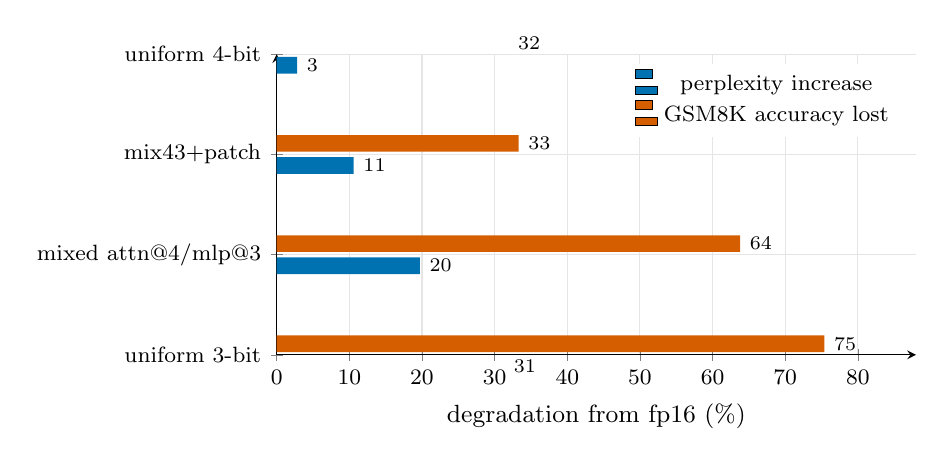
\begin{tikzpicture}
\begin{axis}[
  xbar, width=0.80\linewidth, height=5.4cm,
  xmin=0, xmax=88,
  xlabel={degradation from fp16 (\%)},
  symbolic y coords={uniform 3-bit, mixed attn@4/mlp@3, mix43+patch, uniform 4-bit},
  ytick=data,
  bar width=6pt,
  enlarge y limits=0.22,
  nodes near coords, nodes near coords style={font=\scriptsize},
  nodes near coords align={horizontal},
  every node near coord/.append style={/pgf/number format/precision=0, /pgf/number format/fixed},
  grid=major, grid style={black!10}, axis lines=left,
  tick label style={font=\footnotesize}, label style={font=\small},
  legend style={draw=none, font=\footnotesize, at={(0.98,0.97)}, anchor=north east},
]
\addplot[fill=okblue, draw=none] coordinates
  {(2.8,uniform 4-bit) (10.6,mix43+patch) (19.7,mixed attn@4/mlp@3) (31.3,uniform 3-bit)};
\addplot[fill=okverm, draw=none] coordinates
  {(31.9,uniform 4-bit) (33.3,mix43+patch) (63.8,mixed attn@4/mlp@3) (75.4,uniform 3-bit)};
\legend{perplexity increase, GSM8K accuracy lost}
\end{axis}
\end{tikzpicture}
\caption{Perplexity understates task damage by roughly an order of magnitude
(Qwen2.5-0.5B-Instruct, math). Each configuration's perplexity increase over
fp16 (blue) is dwarfed by its GSM8K accuracy loss (orange): uniform 4-bit costs
only $+2.8\%$ perplexity but $-32\%$ accuracy. A quantization ``recovery''
figure reported in perplexity is systematically optimistic about surviving
capability.}
\label{fig:pplacc}
\end{figure}

Config ordering is identical under both metrics (Fig.~\ref{fig:pplacc}), so
\emph{comparative} conclusions in this paper (and in PTQ work generally) are
safe---with the exception of Sec.~\ref{sec:learned}, where a learned patch
inverts the ranking. But absolute ``gap closed'' or ``$X\%$ recovered''
figures reported in perplexity---ubiquitous in the quantization
literature---overstate how much task capability survives. We recommend
downstream accuracy as a primary metric for sub-4-bit claims.

\subsection{Calibration-seed variance}
Re-running the composite configuration across three disjoint calibration draws
gives relative standard deviations of 0.22\% (knowledge), 1.02\% (chat), 2.07\%
(code), and 3.35\% (math). This is the first such measurement in our study, and
it is consequential: the bitmap encoding's perplexity gain ($+0.6$ to $+2.2\%$)
is within seed noise on two of four tasks. More broadly, \emph{any single-seed
perplexity difference smaller than $\sim$3\% on math should be treated as
unproven}. Bootstrap over evaluation items, standard in this area, captures
evaluation noise but not calibration-draw variance and thus understates
uncertainty.

\section{Limitations}
Experiments center on Qwen2.5-0.5B with scale checks at 1.5B/7B; the frontier
in accuracy is characterized only at 0.5B, where GSM8K accuracy is modest
(34.5\% at \code{fp16}) and the accuracy test resolves only differences of
$\gtrsim$13\% at $n{=}200$---a null result there means ``indistinguishable at
this sample size,'' not ``identical.'' We use fake quantization and claim no
wall-clock speedup; realizing the memory savings requires mixed-precision
kernels we do not implement. We evaluate one downstream task (GSM8K);
broader task coverage, and larger models where accuracy is not floored, are
the clear next steps. Patches store a quantized residual; learned patches
(a QLoRA-style direction) may recover more but blur the comparison to
training-free uniform quantization and are deliberately out of scope.

\section{Conclusion}
Task-conditional precision patches are a real, statistically decisive mechanism
that nonetheless does not beat the simplest baseline of spending bits
uniformly. Their genuine value is geometric: they, and cheap per-layer-type
mixed precision, fill the sub-integer-\bpw{} bands that integer-only uniform
quantization cannot occupy, and a mixed-precision base plus a small
\emph{restored} 3-bit patch ties uniform 4-bit at lower memory on both
perplexity and GSM8K accuracy (Sec.~\ref{sec:frontier}). The robust, deployable
win is the mixed-precision base itself. The task \emph{conditioning}, the
premise of swappability, does not pay: a universal patch works as well as
per-task ones. And the most seductive extension---replacing restoration with an
end-to-end learned patch---is a trap: it wins on perplexity and loses on
accuracy, ending below the unpatched base.

Equally important are the guardrails the study produced: a noise-ceiling
methodology for task-sensitivity claims; a demonstration that perplexity
understates quantization damage by roughly an order of magnitude---and, for the
learned patch, inverts the ranking outright; and a quantification of
calibration-seed variance that retroactively bounds which small ``wins'' in
this space are real. If there is one transferable lesson, it is the discipline
itself: compare at matched memory, interpret overlap against a noise ceiling,
and never let a perplexity number stand as a capability claim without a
downstream check. We release everything, including the negative results and the
retracted claims, in that spirit.

\paragraph{Reproducibility.} All code, experiment scripts, result files, and
the full record of retracted claims are available at
\url{https://github.com/mustafacem/ef_gain}.

\bibliographystyle{ACM-Reference-Format}
\bibliography{refs}

\appendix

\section{Reproducibility Checklist for JAIR}

\subsection*{All articles:}
\begin{enumerate}
    \item All claims investigated in this work are clearly stated. \textbf{yes}
    \item Clear explanations are given how the work reported substantiates the
      claims. \textbf{yes}
    \item Limitations or technical assumptions are stated clearly and
      explicitly. \textbf{yes}
    \item Conceptual outlines and/or pseudo-code descriptions of the AI methods
      introduced in this work are provided, and important implementation
      details are discussed. \textbf{yes}
    \item Motivation is provided for all design choices, including algorithms,
      implementation choices, parameters, data sets and experimental protocols
      beyond metrics. \textbf{yes}
\end{enumerate}

\subsection*{Articles containing theoretical contributions:}
Does this paper make theoretical contributions? \textbf{no}

\subsection*{Articles reporting on computational experiments:}
Does this paper include computational experiments? \textbf{yes}
\begin{enumerate}
    \item All source code required for conducting experiments is included in an
      online appendix or will be made publicly available upon publication.
      \textbf{yes} (\url{https://github.com/mustafacem/ef_gain})
    \item The source code comes with a license that allows free usage for
      reproducibility purposes. \textbf{yes}
    \item The source code comes with a license that allows free usage for
      research purposes in general. \textbf{yes}
    \item Raw, unaggregated data from all experiments is included in an online
      appendix or will be made publicly available. \textbf{yes} (per-experiment
      JSON result files, including per-item GSM8K correctness vectors)
    \item The unaggregated data comes with a license that allows free usage for
      reproducibility purposes. \textbf{yes}
    \item The unaggregated data comes with a license that allows free usage for
      research purposes in general. \textbf{yes}
    \item If an algorithm depends on randomness, then the method used for
      generating random numbers and for setting seeds is described in a way
      sufficient to allow replication of results. \textbf{yes}
    \item The execution environment for experiments, the computing
      infrastructure (hardware and software) used for running them, is
      described. \textbf{yes} (single NVIDIA RTX 4050 laptop GPU, 6\,GB VRAM;
      PyTorch 2.10, CUDA 12.8, Transformers 4.44+, Python 3.12, Linux 6.8;
      exact versions pinned in the repository)
    \item The evaluation metrics used in experiments are clearly explained and
      their choice is explicitly motivated. \textbf{yes} --- indeed the
      relationship between the two metrics is itself a contribution
      (Sec.~\ref{sec:caveats}).
    \item The number of algorithm runs used to compute each result is reported.
      \textbf{yes}
    \item Reported results have not been ``cherry-picked'' by silently ignoring
      unsuccessful or unsatisfactory experiments. \textbf{yes} --- rejected
      ideas are reported in Sec.~\ref{sec:negative} with their pre-registered
      promotion rules, and four claims made during the study are explicitly
      retracted.
    \item Analysis of results goes beyond single-dimensional summaries of
      performance to include measures of variation, confidence, or other
      distributional information. \textbf{yes} (paired bootstrap over
      evaluation items throughout; calibration-seed variance quantified in
      Sec.~\ref{sec:caveats})
    \item All (hyper-)parameter settings for the algorithms/methods used in
      experiments have been reported, along with the rationale or method for
      determining them. \textbf{yes}
    \item The number and range of (hyper-)parameter settings explored prior to
      conducting final experiments have been indicated, along with the effort
      spent on (hyper-)parameter optimisation. \textbf{partially} --- the
      patch-precision, budget, coverage and training-data sweeps are reported
      in full; the learning-rate search for the learned patch is reported only
      as the final setting plus the one divergent value that motivated it.
    \item Appropriately chosen statistical hypothesis tests are used to
      establish statistical significance in the presence of noise effects.
      \textbf{yes}
\end{enumerate}

\subsection*{Articles using data sets:}
Does this work rely on one or more data sets? \textbf{yes}
\begin{enumerate}
    \item All newly introduced data sets are included in an online appendix or
      will be made publicly available. \textbf{NA} --- no new data sets are
      introduced.
    \item The newly introduced data set comes with a license that allows free
      usage for reproducibility purposes. \textbf{NA}
    \item The newly introduced data set comes with a license that allows free
      usage for research purposes in general. \textbf{NA}
    \item All data sets drawn from the literature or other public sources are
      accompanied by appropriate citations. \textbf{yes} (MBPP, GSM8K,
      ARC-Easy, WikiText-2, CodeParrot)
    \item All data sets drawn from the existing literature are publicly
      available. \textbf{yes}
    \item All new data sets and data sets that are not publicly available are
      described in detail. \textbf{NA}
    \item All methods used for preprocessing, augmenting, batching or splitting
      data sets are described in detail. \textbf{yes} (2048-token
      concatenate-and-chunk calibration, calibration/evaluation split by
      corpus or split, 8-gram leakage check reported)
\end{enumerate}

\subsection*{Explanations on any of the answers above (optional):}

Results are single-seed with respect to the calibration draw; we quantify that
variance (up to 3.35\% relative on math) and state explicitly in
Sec.~\ref{sec:caveats} which reported differences fall below it and should
therefore be treated as unproven. Absolute perplexities are not comparable
across tables because evaluation sequence length differs between experiments;
every comparison and significance test is within a single run, as noted in
Sec.~\ref{sec:setup}.

\end{document}
